%definira klasu dokumenta 
\documentclass[12pt]{report} 

%prostor izmedu naredbi \documentclass i \begin{document} se zove uvod. U njemu se nalaze naredbe koje se odnose na cijeli dokument

%osnovni LaTex ne može riješiti sve probleme, pa se koriste različiti paketi koji olakšavaju izradu željenog dokumenta
\usepackage[croatian]{babel} 
\usepackage{amssymb}
\usepackage{amsmath}
\usepackage{txfonts}
\usepackage{mathdots}
\usepackage{titlesec}
\usepackage{array}
\usepackage{lastpage}
\usepackage{etoolbox}
\usepackage{tabularray}
\usepackage{color, colortbl}
\usepackage{adjustbox}
\usepackage{geometry}
\usepackage[classicReIm]{kpfonts}
\usepackage{hyperref}
\usepackage{fancyhdr}

\usepackage{float}
\usepackage{setspace}
\restylefloat{table}


\patchcmd{\chapter}{\thispagestyle{plain}}{\thispagestyle{fancy}}{}{} %redefiniranje stila stranice u paketu fancyhdr

%oblik naslova poglavlja
\titleformat{\chapter}{\normalfont\huge\bfseries}{\thechapter.}{20pt}{\Huge}
\titlespacing{\chapter}{0pt}{0pt}{40pt}


\linespread{1.3} %razmak između redaka

\geometry{a4paper, left=1in, top=1in,}  %oblik stranice

\hypersetup{ colorlinks, citecolor=black, filecolor=black, linkcolor=black,	urlcolor=black }   %izgled poveznice


%prored smanjen između redaka u nabrajanjima i popisima
\newenvironment{packed_enum}{
	\begin{enumerate}
		\setlength{\itemsep}{0pt}
		\setlength{\parskip}{0pt}
		\setlength{\parsep}{0pt}
	}{\end{enumerate}}

\newenvironment{packed_item}{
	\begin{itemize}
		\setlength{\itemsep}{0pt}
		\setlength{\parskip}{0pt}
		\setlength{\parsep}{0pt}
	}{\end{itemize}}




%boja za privatni i udaljeni kljuc u tablicama
\definecolor{LightBlue}{rgb}{0.9,0.9,1}
\definecolor{LightGreen}{rgb}{0.9,1,0.9}

%Promjena teksta za dugačke tablice
\DefTblrTemplate{contfoot-text}{normal}{Nastavljeno na idućoj stranici}
\SetTblrTemplate{contfoot-text}{normal}
\DefTblrTemplate{conthead-text}{normal}{(Nastavljeno)}
\SetTblrTemplate{conthead-text}{normal}
\DefTblrTemplate{middlehead,lasthead}{normal}{Nastavljeno od prethodne stranice}
\SetTblrTemplate{middlehead,lasthead}{normal}

%podesavanje zaglavlja i podnožja

\pagestyle{fancy}
\lhead{Programsko inženjerstvo}
\rhead{$<$Projektni zadatak$>$}
\lfoot{$<$Naziv grupe$>$}
\cfoot{stranica \thepage/\pageref{LastPage}}
\rfoot{\today}
\renewcommand{\headrulewidth}{0.2pt}
\renewcommand{\footrulewidth}{0.2pt}

\graphicspath{ {./slike/} }


\begin{document} 
	
	
	
	\begin{titlepage}
		\begin{center}
			\vspace*{\stretch{1.0}} %u kombinaciji s ostalim \vspace naredbama definira razmak između redaka teksta
			\LARGE Programsko inženjerstvo\\
			\large Ak. god. 2020./2021.\\
			
			\vspace*{\stretch{3.0}}
			
			\huge $<$Naziv projekta$>$\\
			\Large Dokumentacija, Rev. \textit{$<$1 ili 2$>$}\\
			
			\vspace*{\stretch{12.0}}
			\normalsize
			Grupa: \textit{$<$Naziv grupe$>$}\\
			Voditelj: \textit{$<$Ime i prezime voditelja$>$}\\
			
			
			\vspace*{\stretch{1.0}}
			Datum predaje: \textit{$<$dan$>$. $<$mjesec$>$. $<$godina$>$.}\\
	
			\vspace*{\stretch{4.0}}
			
			Nastavnik: \textit{$<$Ime i prezime nastavnika zaduženog za vašu grupu$>$}\\
		
		\end{center}

	
	\end{titlepage}

	
	\tableofcontents


	\chapter{Dnevnik promjena dokumentacije}
		
		\textbf{\textit{Kontinuirano osvježavanje}}\\
				
		
		\begin{longtblr}[
				label=none
			]{
				width = \textwidth, 
				colspec={|X[2]|X[13]|X[3]|X[3]|}, 
				rowhead = 1
			}
			\hline
			\textbf{Rev.}	& \textbf{Opis promjene/dodatka} & \textbf{Autori} & \textbf{Datum}\\[3pt] \hline
			0.1 & Napravljen predložak.	& Agejev & 30.10.2023. 		\\[3pt] \hline
			0.2 & Dodani obrasci uporabe, dijagrami obrazaca uporabe, akteri i dionici. & Skukan & 29.10.2023. \\[3pt] \hline 
			0.3	& Opis projektnog zadatka & Agejev, Haralović & 02.11.2023. 	\\[3pt] \hline
			0.4	& Dijagram razreda & Vidović & 03.11.2023. 	\\[3pt] \hline
			0.5	& Opis baze podataka & Tomić & 05.11.2023. 	\\[3pt] \hline
			0.6 & Prva inačica sekvencijskih dijagrama & Lovrinović & 6.11.2023. \\[3pt] \hline
			0.7 & Ostali zahtjevi & Agejev & 7.11.2023. \\[3pt] \hline
			0.8 & Prepravljeni sekvencijski dijagrami. \newline Dodano opcionalno filtriranje. & Skukan & 9.11.2023. \\[3pt] \hline
			0.9 & Prepravljeni obrasci uporabe i dijagrami. \newline Maknut UC17. & Skukan & 14.11.2023. \\[3pt] \hline
			0.10 & Ispravci kod aktera i obrazaca. \newline Nova slika dijagrama obrazaca. & Skukan & 16.11.2023. \\[3pt] \hline
			& & \\[3pt] \hline
			0.8 & Povijest rada i trenutni status implementacije,\newline Zaključci i plan daljnjeg rada & * & 28.08.2013. \\[3pt] \hline 
			0.9 & Opisi obrazaca uporabe & * & 07.09.2013. \\[3pt] \hline 
			0.10 & Preveden uvod & * & 08.09.2013. \\[3pt] \hline 
			0.11 & Sekvencijski dijagrami & * & 09.09.2013. \\[3pt] \hline 
			0.12.1 & Započeo dijagrame razreda & * & 10.09.2013. \\[3pt] \hline 
			0.12.2 & Nastavak dijagrama razreda & * & 11.09.2013. \\[3pt] \hline 
			\textbf{1.0} & Verzija samo s bitnim dijelovima za 1. ciklus & * & 11.09.2013. \\[3pt] \hline 
			1.1 & Uređivanje teksta -- funkcionalni i nefunkcionalni zahtjevi & * \newline * & 14.09.2013. \\[3pt] \hline 
			1.2 & Manje izmjene:Timer - Brojilo vremena & * & 15.09.2013. \\[3pt] \hline 
			1.3 & Popravljeni dijagrami obrazaca uporabe & * & 15.09.2013. \\[3pt] \hline 
			1.5 & Generalna revizija strukture dokumenta & * & 19.09.2013. \\[3pt] \hline 
			1.5.1 & Manja revizija (dijagram razmještaja) & * & 20.09.2013. \\[3pt] \hline 
			\textbf{2.0} & Konačni tekst predloška dokumentacije  & * & 28.09.2013. \\[3pt] \hline 
			&  &  & \\[3pt] \hline	
		\end{longtblr}
	
	
		\textit{Moraju postojati glavne revizije dokumenata 1.0 i 2.0 na kraju prvog i drugog ciklusa. Između tih revizija mogu postojati manje revizije već prema tome kako se dokument bude nadopunjavao. Očekuje se da nakon svake značajnije promjene (dodatka, izmjene, uklanjanja dijelova teksta i popratnih grafičkih sadržaja) dokumenta se to zabilježi kao revizija. Npr., revizije unutar prvog ciklusa će imati oznake 0.1, 0.2, …, 0.9, 0.10, 0.11.. sve do konačne revizije prvog ciklusa 1.0. U drugom ciklusu se nastavlja s revizijama 1.1, 1.2, itd.}
	\chapter{Opis projektnog zadatka}
		
		
		Namjera projekta riješiti je trenutačan manjak strane literature prevedene na hrvatski ili srodni jezik. Količina kvalitetne literature ograničena je i često teško dostupna u Hrvatskoj, dok web poslužitelji i stranice ne nude centralizirano rješenje za pronalazak domaćih izdanja niti jednostavnu opciju zahtjeva novih prijevoda. Naime, web stranice raznih antikvarijata nisu ažurne, metode pretraživanja nezgrapne su, a u katalogu imaju popis knjiga koji ne odgovara trenutačnom stanju u njihovim skladištima. Mnogo knjiga u njihovoj ponudi nije prevedena ili ne sadrži naslov izvornika čime je nabava željene knjige otežana.
		
		Svojim rješenjem nadamo se olakšati krajnjem korisniku pretragu i nabavku željene knjige, osobito domaćih izdanja. Naše rješenje temelji se na izradi web stranice koja služi kao posrednik između ponuditelja i korisnika, s ažurnom bazom knjiga koja brojčano nadmašuje ostale stranice. 
		
		Poseban naglasak stavljamo na literaturu prevedenu na hrvatski i jezike slične hrvatskom, a korisnicima pojednostavljujemo proces pronalaska i odabira željenog naslova dostupnošću raznovrsnih ponuditelja (izdavačkih kuća, preprodavača, antikvarijata).
		
		Web stranica služila bi kao središnje mjesto ponude različitih izdavačkih kuća, manjih knjižara i individualnih preprodavača, na taj način stvarajući veću ponudu, bolju pokrivenost i konkurentnije cijene krajnjem korisniku.
		
		Krajnjem korisniku olakšavamo pregled trenutno dostupnih knjiga na hrvatskom, srodnim i stranim jezicima. Nudimo lokacijsku preglednost ponude određenog naslova, odnosno informaciju o dostupnosti na stranom tržištu, ukoliko je knjiga nedostupna na lokalnom području.
		
		Također nudimo mogućnost zahtjeva prijevoda knjige ovisno o interesima korisnika, izdavač može ostvariti kontakt s izdavačem strane knjige i ishodovati dozvolu za prijevod knjige na jezik blizak krajnjem korisniku.\\
		
		
		
		\subsection{Slična rješenja}
		
		Trenutno je tržište knjiga u velikoj mjeri digitalizirano. Naravno, i dalje postoje knjižare te knjige se i dalje kupuju u fizičkom obliku, ali većina izdavačkih kuća nudi svoj asortiman na web stranicama. Mnoge izdavačke kuće prenijele su dio svoje ponude na web, što je jasan pokazatelj korisničkog interesa za sličnim rješenjima.
		
		Tako, na primjer, Naklada Znanje na svom portalu nudi knjige podijeljene u kategorije knjiga prevedenih na hrvatski te strane knjige, većinom na engleskom jeziku. Njihov asortiman nije ograničen samo na knjige; imaju i kategorije poput igračaka, multimedije i slično. Na slici 2.1 vidimo njihovu web stranicu.
		
		\begin{figure}[H]
			
\includegraphics[scale=1]{slike/naklada-znanje.PNG} %veličina slike u odnosu na originalnu datoteku i pozicija slike
			\centering
			\caption{web stranica naklade \textit{Znanje}}
			\label{fig:Naklada Znanje}
		\end{figure}
		
		Na njihovoj stranici možete pretraživati knjige po naslovu, autoru ili ključnim riječima, a omogućena je i jednostavna kupovina.
		
		Eknjiga.hr nudi slično rješenje, s tom razlikom da na njihovoj stranici korisnik može odabrati i izdavača u sekciji "Izdavač", omogućavajući tako izdavačima i korisnicima da lakše pristupe ponudi knjiga. Takva ponuda sliči rješenju koje mi nudimo, odnosno centraliziranom i neovisnom posredniku između ponuditelja i korisnika.
		
		Na slici 2.2 vidimo njihovo rješenje:
		
		\begin{figure}[H]
			\includegraphics[scale=1]{slike/Eknjiga.PNG} %veličina slike u odnosu na originalnu datoteku i pozicija slike
			\centering
			\caption{web stranica \textit{Eknjiga.hr}}
			\label{fig:Eknjiga}
		\end{figure}
		
		
		Zbog sličnosti s gore navedenim, nećemo dodatno opisivati slične portale i stranice, ali ih ovdje navodimo: Mozaik knjiga, Školska knjiga, Super knjižara, Hoću knjigu, VBZ knjižara, Knjiga HR, Čitaj knjigu, Svijet knjige, Libristo, Profil knjiga, E-knjižara i mnogi drugi. Također, knjige se nude i na aplikacijama poput Njuškala.
		
		Naše rješenje razlikuje se po nekoliko aspekata. Većina postojećih platformi nudi kategorijsku podjelu knjiga, promotivne akcije i ponude usmjerene korisnicima koji ciljano pristupaju tim knjižarama kako bi pronašli određeni naslov ili se izložili širokoj ponudi te time možda pronašli knjigu od interesa. Taj pristup je usmjeren prema promociji cjelokupne ponude određenog izdavača ili nakladnika, s ciljem privlačenja korisnika na kupnju kod njih. 
		
		S druge strane, naša platforma nije posvećena jednom izdavaču, ali ne dozvoljava ni neprovjerene i privatne prodavače. Umjesto toga, dizajnirana je s korisnikom u središtu pažnje, omogućavajući mu da na temelju lokacije, jezika i naslova pronađe knjigu po najpovoljnijim uvjetima kupnje – bilo da je to cjenovna prihvatljivost, pogodna lokacija kupovine ili povjerenje u izdavača.
		
		\subsection{Ciljana publika}
		
		Naša stranica namijenjena je svima koji žele kupiti knjigu, a osobito onima koji ne znaju strane jezike ili radije čitaju na materinjem ili srodnom jeziku. Ponuditeljima stranica nudi uvid u želje kupaca putem skupljanja zahtjeva za prijevode te platformu za prodaju.
		
		Uzimajući u obzir korisnika koji ima preferira određenog izdavača u odnosu na ostale, teško je za očekivati kako će se isti odlučiti za promjenom i našim rješenjem ukoliko odabrani naslov koji traži može pronaći kod tog izdavača.
		
		Naša web stranica namijenjena je sljedećim tipovima kupaca:
		
		\begin{packed_enum}
			\item korisniku sa specifičnim zahtjevom knjige na preferiranom jeziku ili određenoj lokaciji, kojemu je u interesu pronaći knjigu koju možebitno nema u katalogu izdavača od povjerenja
			\item korisniku koji po lokaciji i odabranom jeziku želi pregledati ponudu knjiga koje bi ga mogle zanimati
			\item neodlučnom korisniku koji nije siguran u odabir knjige (cijena, udaljenost izdavača)
		\end{packed_enum}
		
		Registriranim ponuditeljima naša stranica nudi:	
		
		\begin{packed_enum}
			\item stranicu sa značajkama atraktivnim kupcima
			\item izbjegavanje potrebe vlastitog web rješenja
			\item mogućnošću prodaje knjiga koje su rijetko kupovane te su ispale iz glavne ponude
			\item uvid u želje korisnika za prijevodima
		\end{packed_enum}
		
		
		
		
		
		
		\section{Primjeri u \LaTeX u}
		
		\textit{Ovo potpoglavlje izbrisati.}\\

		U nastavku se nalaze različiti primjeri kako koristiti osnovne funkcionalnosti \LaTeX a koje su potrebne za izradu dokumentacije. Za dodatnu pomoć obratiti se asistentu na projektu ili potražiti upute na sljedećim web sjedištima:
		\begin{itemize}
			\item Upute za izradu diplomskog rada u \LaTeX u - \url{https://www.fer.unizg.hr/_download/repository/LaTeX-upute.pdf}
			\item \LaTeX\ projekt - \url{https://www.latex-project.org/help/}
			\item StackExchange za Tex - \url{https://tex.stackexchange.com/}\\
		
		\end{itemize} 	


		
		\noindent \underbar{podcrtani tekst}, \textbf{podebljani tekst}, 	\textit{nagnuti tekst}\\
		\noindent \normalsize primjer \large primjer \Large primjer \LARGE {primjer} \huge {primjer} \Huge primjer \normalsize
				
		\begin{packed_item}
			
			\item  primjer
			\item  primjer
			\item  primjer
			\item[] \begin{packed_enum}
				\item primjer
				\item[] \begin{packed_enum}
					\item[1.a] primjer
					\item[b] primjer
				\end{packed_enum}
				\item primjer
			\end{packed_enum}
			
		\end{packed_item}
		
		\noindent primjer url-a: \url{https://www.fer.unizg.hr/predmet/proinz/projekt}
		
		\noindent posebni znakovi: \# \$ \% \& \{ \} \_ 
		$|$ $<$ $>$ 
		\^{} 
		\~{} 
		$\backslash$ 
		
		
		\begin{longtblr}[
			label=none,
			entry=none
			]{
				width = \textwidth,
				colspec={|X[8,l]|X[8, l]|X[16, l]|}, 
				rowhead = 1,
			} %definicija širine tablice, širine stupaca, poravnanje i broja redaka naslova tablice
			\hline \SetCell[c=3]{c}{\textbf{naslov unutar tablice}}	 \\ \hline[3pt]
			\SetCell{LightGreen}IDKorisnik & INT	&  	Lorem ipsum dolor sit amet, consectetur adipiscing elit, sed do eiusmod  	\\ \hline
			korisnickoIme	& VARCHAR &   	\\ \hline 
			email & VARCHAR &   \\ \hline 
			ime & VARCHAR	&  		\\ \hline 
			\SetCell{LightBlue} primjer	& VARCHAR &   	\\ \hline 
		\end{longtblr}
		

		\begin{longtblr}[
				caption = {Naslov s referencom izvan tablice},
				entry = {Short Caption},
			]{
				width = \textwidth, 
				colspec = {|X[8,l]|X[8,l]|X[16,l]|}, 
				rowhead = 1,
			}
			\hline
			\SetCell{LightGreen}IDKorisnik & INT	&  	Lorem ipsum dolor sit amet, consectetur adipiscing elit, sed do eiusmod  	\\ \hline
			korisnickoIme	& VARCHAR &   	\\ \hline 
			email & VARCHAR &   \\ \hline 
			ime & VARCHAR	&  		\\ \hline 
			\SetCell{LightBlue} primjer	& VARCHAR &   	\\ \hline 
		\end{longtblr}
	


		
		
		%unos slike
		\begin{figure}[H]
			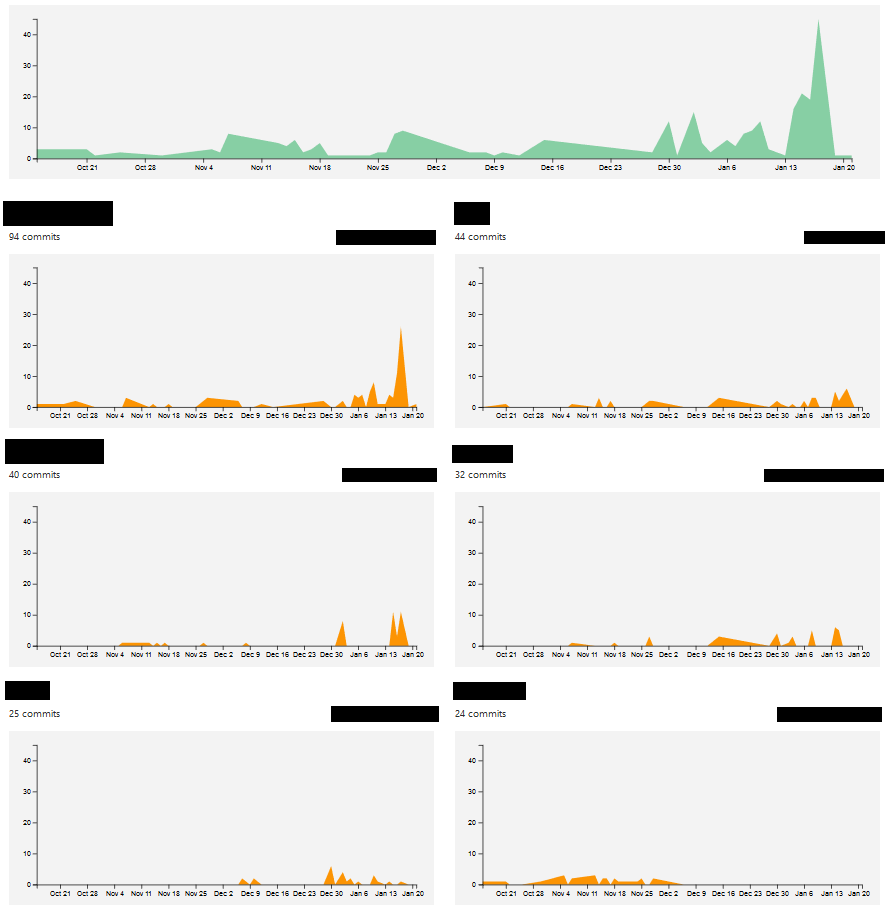
\includegraphics[scale=0.4]{slike/aktivnost.PNG} %veličina slike u odnosu na originalnu datoteku i pozicija slike
			\centering
			\caption{Primjer slike s potpisom}
			\label{fig:promjene}
		\end{figure}
		
		\begin{figure}[H]
			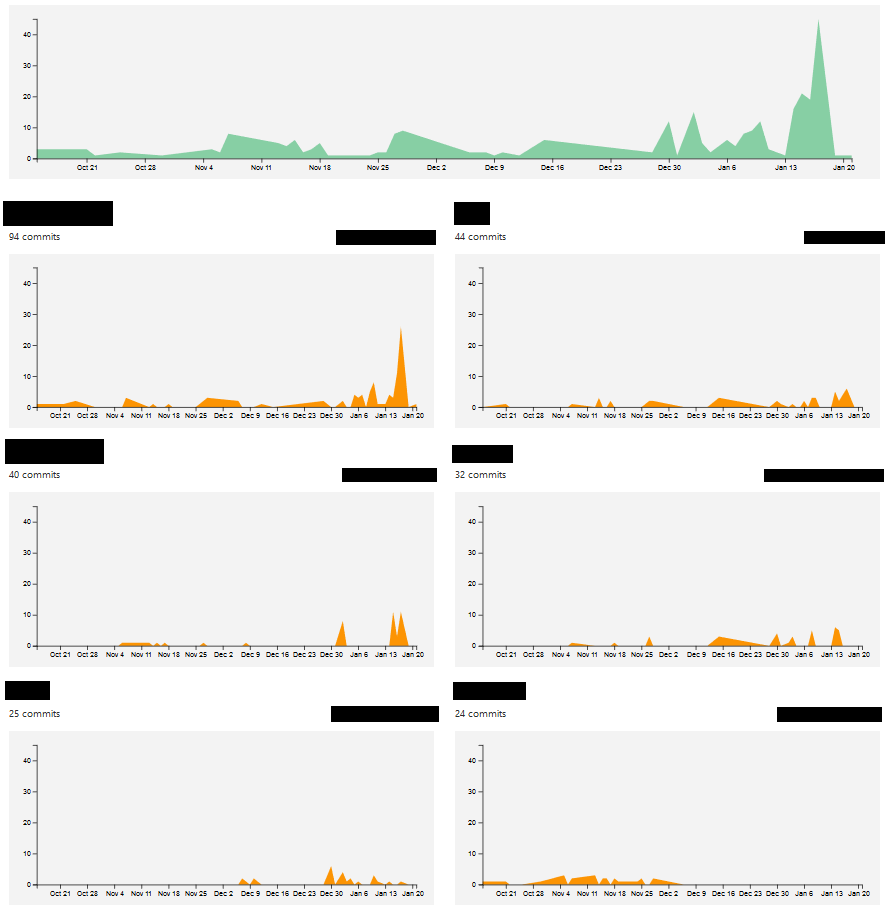
\includegraphics[width=\textwidth]{slike/aktivnost.PNG} %veličina u odnosu na širinu linije
			\caption{Primjer slike s potpisom 2}
			\label{fig:promjene2} %label mora biti drugaciji za svaku sliku
		\end{figure}
		
		Referenciranje slike \ref{fig:promjene2} u tekstu.
		
		\eject
		
	
	\chapter{Specifikacija programske potpore}
		
	\section{Funkcionalni zahtjevi}
			
			\noindent \textbf{Dionici:}
			
			\begin{packed_enum}
				
				\item Klijent
				\item Registrirani korisnik/Ponuditelj		
				\begin{packed_enum}
                    				\item Izdavač
                    				\item Preprodavač
                   				\item Antikvarijat
                			\end{packed_enum}
                			\item Strani izdavač
                			\item Razvojni tim
			\end{packed_enum}
			
			\noindent \textbf{Akteri i njihovi funkcionalni zahtjevi:}
			
			
			\begin{packed_enum}

				 \item \underbar{Korisnik (inicijator) može:}
                
                    				\begin{packed_enum}
                        				\item Pretraživati knjige po njihovim atributima i po ponuditeljima
                        				\item Pregledavati objave
                        				\item Pregledavati profil ponuditelja
					      	\item Pretraživati na karti ponuditelje                      				
                    				\end{packed_enum}
				\item  \underbar{Neregistrirani korisnik(inicijator) može:}
				
				\begin{packed_enum}
					\item Napraviti korisnički račun registracijom za što mu treba korisničko ime, lozinka, e-mail, broj mobitela i adresa i može birati u koju će kategoriju ponuditelja spadati
					\item Slati zahtjev izdavačima da se knjiga na stranom jeziku prevede		
				\end{packed_enum}
			
				\item  \underbar{Registrirani korisnik tj. ponuditelj (izdavač/antikvarijat/preprodavač)(inicijator) može:}
				
				\begin{packed_enum}
					
					\item Prijaviti se u sustav koristeći korisničko ime i lozinku
                   				\item Pregledavati svoj račun, mijenjati njegove podatke i izbrisati ga
					\item Stavljati , mijenjati i brisati njegove objave za knjige
					
				\end{packed_enum}

				\item \underbar{Izdavač (inicijator) može:}

                				\begin{packed_enum}
                    					\item Slati zahtjev za prijevod knjige stranom izdavaču
                				\end{packed_enum}

                			\item \underbar{Administrator(sudionik):}
                			\begin{packed_enum}
                    				\item Prima zahtjev za registraciju i na temelju unesenih podataka potvrđuje ili odbija registraciju
                			\end{packed_enum}

                			\item \underbar{Strani izdavač(sudionik):}
                			\begin{packed_enum}
                    				\item Prima zahtjev od strane izdavača za prijevod knjige
                			\end{packed_enum}

                			\item \underbar{Baza podataka(sudionik):}
                			\begin{packed_enum}
                    				\item Pohranjuje podatke o korisnicima i njihovim ovlastima
                    				\item Pohranjuje podatke o objavljenim knjigama
                			\end{packed_enum}
			\end{packed_enum}
			
			\eject 
			
			
			\subsection{Obrasci uporabe}
				

				
				\subsubsection{Opis obrazaca uporabe}				
					\noindent \underbar{\textbf{UC1 - Registracija}}
            
					\begin{packed_item}

						\item  \textbf{Glavni sudionik: } Neregistrirani korisnik
						\item  \textbf{Cilj:} Izrada korisničkog računa za web stranicu
						\item  \textbf{Sudionici:} Baza podataka
						\item  \textbf{Preduvjet:} -
						\item  \textbf{Opis osnovnog tijeka:}
						
						\item[] \begin{packed_enum}
	
							\item Neregistrirani korisnik bira opciju registracije
                           					\item Unosi podatke potrebne za registraciju
							\item Web obavještava korisnika da će zahtjev za registraciju pregledati administrator
						\end{packed_enum}
						
						\item  \textbf{Opis mogućih odstupanja:}
						
						\item[] \begin{packed_item}
	
							\item[2.a] Korisnik unosi zauzeto korisničko ime, e-mail ili broj telefona ili je neki od podataka u krivom formatu
							\item[] \begin{packed_enum}
								
								\item Sustav obavještava o neuspjeloj registraciji i gdje je došlo do greške
								\item Korisnik unosi prihvatljive podatke ili odustane od registracije
								
							\end{packed_enum}
						\end{packed_item}
					\end{packed_item}

                    \noindent \underbar{\textbf{UC2- Prijava}}
					\begin{packed_item}
	
						\item \textbf{Glavni sudionik: } Ponuditelj
						\item  \textbf{Cilj:} Dobiti pristup web stranici sa postojećim korisničkim računom
						\item  \textbf{Sudionici:} Baza podataka
						\item  \textbf{Preduvjet:} - Ponuditelj ima izrađen korisnički račun
						\item  \textbf{Opis osnovnog tijeka:}
						
						\item[] \begin{packed_enum}	
							\item Ponuditelj bira opciju prijave
							\item Ponuditelj unosi korisničko ime i lozinku
                            					\item Ponuditelj dobiva pristup svom korisničkom računu
						\end{packed_enum}
						
						\item  \textbf{Opis mogućih odstupanja:}
						
						\item[] \begin{packed_item}
	
							\item[2.a] Jedan ili više potrebnih podataka je krivo uneseno
							\item[] \begin{packed_enum}
								
								\item Sustav obavještava o neuspjeloj prijavi i gdje je došlo do greške
								\item Ponuditelj unosi prihvatljive podatke ili odustane od prijave
								
							\end{packed_enum}
						\end{packed_item}
					\end{packed_item}

                    \noindent \underbar{\textbf{UC3 - Potvrda registracije}}
					\begin{packed_item}
	
						\item \textbf{Glavni sudionik: } Administrator
						\item  \textbf{Cilj:} Potvrđivanje uspješne/neuspješne registracije ponuditelja
						\item  \textbf{Sudionici:} Baza podataka, neregistrirani korisnik
						\item  \textbf{Preduvjet:} - Neregistrirani korisnik pokušava izvršiti registraciju
						\item  \textbf{Opis osnovnog tijeka:}
						
						\item[] \begin{packed_enum}	
							\item Nakon što korisnik unese podatke za registraciju, zahtjev za registraciju se šalje administratoru na pregled
							\item Provjerava se da su uneseni podaci dobrog oblika i da ne postoje u bazi podataka
                           					\item Administrator potvrđuje unesene podatke i informira da je registracija uspješna
						\end{packed_enum}
						
						\item  \textbf{Opis mogućih odstupanja:}
						
						\item[] \begin{packed_item}
	
							\item[2.a] Podaci su krivog formata ili već upisani u bazu podataka jer ih netko drugi koristi
							\item[] \begin{packed_enum}			
								\item Administrator obavještava da je došlo do greške i zašto
							\end{packed_enum}
						\end{packed_item}
					\end{packed_item}

                    \noindent \underbar{\textbf{UC4 - Biranje kategorije ponuditelja}}
					\begin{packed_item}
	
						\item \textbf{Glavni sudionik: } Neregistrirani korisnik
						\item  \textbf{Cilj:} Biranje kategorije ponuditelja u koju će spadati korisnički račun
						\item  \textbf{Sudionici:} Baza podataka
						\item  \textbf{Preduvjet:} - Korisnik je započeo registraciju
						\item  \textbf{Opis osnovnog tijeka:}
						
						\item[] \begin{packed_enum}
	
							\item Pri registraciji korisnik klikne na polje kojim bira u koju će kategoriju spadati
							\item Korisnik bira kategoriju i nastavlja sa registracijom
						\end{packed_enum}
						
						\item  \textbf{Opis mogućih odstupanja:-}
					
					\end{packed_item}

                    \noindent \underbar{\textbf{UC5 - Pregled korisničkog računa}}
					\begin{packed_item}
	
						\item \textbf{Glavni sudionik: } Ponuditelj
						\item  \textbf{Cilj:} Ponuditelj pregledava podatke o svom korisničkom računu
						\item  \textbf{Sudionici:} Baza podataka
						\item  \textbf{Preduvjet:} - Ponuditelj je prijavljen
						\item  \textbf{Opis osnovnog tijeka:}
						
						\item[] \begin{packed_enum}
	
							\item Ponuditelj bira opciju "Moj račun"
							\item Aplikacija prikazuje pripadni korisnički račun i podatke
						\end{packed_enum}
						
						\item  \textbf{Opis mogućih odstupanja: -}
						
					\end{packed_item}

                    \noindent \underbar{\textbf{UC6 - Promjena podataka}}
					\begin{packed_item}
	
						\item \textbf{Glavni sudionik: } Ponuditelj
						\item  \textbf{Cilj:} Ponuditelj mijenja podatke svog korisničkog računa
						\item  \textbf{Sudionici:} Baza podataka
						\item  \textbf{Preduvjet:} - Ponuditelj je prijavljen
						\item  \textbf{Opis osnovnog tijeka:}
						
						\item[] \begin{packed_enum}
	
							\item Ponuditelj bira opciju "Moj račun"
							\item Ponuditelj bira opciju "Uredi račun"
	                            				\item Ponuditelj mijenja podatke
                            					\item Ponuditelj sprema izmjene
                            					\item Baza podataka se ažurira
						\end{packed_enum}
						
						\item  \textbf{Opis mogućih odstupanja:}
						
						\item[] \begin{packed_item}
	
							\item[2.a] Ponuditelj unosi podatke u krivom formatu ili su podaci već korišteni od strane drugih ponuditelja
							\item[] \begin{packed_enum}
								
								\item Aplikacija obavještava da je došlo do greške i zašto
								\item Ponuditelj opet pokušava promijeniti podatke ili odustaje
							\end{packed_enum}

                            					\item[2.b] Ponuditelj upisuje nove podatke ali ne klikne na opciju spremanja promjena
                            					\item[] \begin{packed_enum}
                                					\item Aplikacija obavještava da promjene nisu pohranjene
                            					\end{packed_enum}
						\end{packed_item}
					\end{packed_item}

                    \noindent \underbar{\textbf{UC7 - Brisanje korisničkog računa}}
					\begin{packed_item}
	
						\item \textbf{Glavni sudionik: } Ponuditelj
						\item  \textbf{Cilj:} Ponuditelj briše svoj račun sa web stranice
						\item  \textbf{Sudionici:} Baza podataka
						\item  \textbf{Preduvjet:} - Ponuditelj ima izrađen korisnički račun
						\item  \textbf{Opis osnovnog tijeka:}
						
						\item[] \begin{packed_enum}
	
							\item Ponuditelj bira opciju "Moj račun"
                            					\item Ponuditelj bira opciju brisanja korisničkog računa
							\item Aplikacija traži potvrdu brisanja
                            					\item Ponuditelj potvrđuje brisanje korisničkog računa
                            					\item Miču se podaci o računu iz baze podataka
                            					\item Ponuditelj je vraćen na stranicu za upis
						\end{packed_enum}
						
						\item  \textbf{Opis mogućih odstupanja: -}
					\end{packed_item}

                    \noindent \underbar{\textbf{UC8 - Dodavanje objave}}
					\begin{packed_item}
	
						\item \textbf{Glavni sudionik: } Ponuditelj
						\item  \textbf{Cilj:} Dodavanje objave knjige za prodaju na web stranicu
						\item  \textbf{Sudionici:} Baza podataka
						\item  \textbf{Preduvjet:} - Ponuditelj je prijavljen
						\item  \textbf{Opis osnovnog tijeka:}
						
						\item[] \begin{packed_enum}
	
							\item Ponuditelj bira opciju "Nova objava"
                            					\item Aplikacija otvara stranicu za novu objavu
                            					\item Ponuditelj unosi potrebne podatke
							\item Ponuditelj klikne opciju "Objavi"
                            					\item Objava knjige je vidljiva na web stranici i u bazi podataka
						\end{packed_enum}
						
						\item  \textbf{Opis mogućih odstupanja:}
						
						\item[] \begin{packed_item}
	
							\item[2.a] Ponuditelj unosi krivi format podataka potrebnih za objavu
							\item[] \begin{packed_enum}
								
								\item Aplikacija obavještava da je format kriv i gdje
								\item Ponuditelj unosi prihvatljive podatke ili odustaje od objave
							\end{packed_enum}
                            					\item[2.b] Ponuditelj ne unosi sve potrebne podatke da se napravi objava
                             					\item[] \begin{packed_enum}
                                 					\item Aplikacija obavještava da jedno ili više polja nije popunjeno
                                 					\item Ponuditelj popunjuje prazna polja ili odustaje od objave
                             					\end{packed_enum}
						\end{packed_item}
					\end{packed_item}

                    \noindent \underbar{\textbf{UC9 - Mijenjanje objave}}
					\begin{packed_item}
	
						\item \textbf{Glavni sudionik: } Ponuditelj
						\item  \textbf{Cilj:} Mijenjanje podataka objave za knjigu
						\item  \textbf{Sudionici:} Baza podataka
						\item  \textbf{Preduvjet:} - Postoji objava za knjigu
						\item  \textbf{Opis osnovnog tijeka:}
						
						\item[] \begin{packed_enum}	
							\item Ponuditelj klikne na objavu koju želi promijeniti
                            					\item Aplikacija otvara stranicu objave
							\item Ponuditelj bira opciju mijenjanja podataka
                            					\item Ponuditelj izmjenjuje podatke
                            					\item Ponuditelj sprema izmjene
                            					\item Novi podaci su zapisani u bazu podataka
						\end{packed_enum}
						
						\item  \textbf{Opis mogućih odstupanja:}
						
						\item[] \begin{packed_item}
	
							\item[2.a] Ponuditelj unosi podatke u krivom formatu
							\item[] \begin{packed_enum}
								
								\item Aplikacija obavještava gdje je došlo do greške i zašto
								\item Ponuditelj unosi prihvatljive podatke ili odustane od izmjene podataka
								
							\end{packed_enum}

                            					\item[2.b] Ponuditelj ne sprema izmjene
                            					\item[] \begin{packed_enum}
                                					\item Aplikacija obavještava da promjene nisu pohranjene	
                            					\end{packed_enum}
						\end{packed_item}
					\end{packed_item}

                    \noindent \underbar{\textbf{UC10 - Brisanje objave}}
					\begin{packed_item}
	
						\item \textbf{Glavni sudionik: } Ponuditelj
						\item  \textbf{Cilj:} Ponuditelj briše svoju objavu
						\item  \textbf{Sudionici:} Baza podataka
						\item  \textbf{Preduvjet:} - Ponuditelj ima objavu
						\item  \textbf{Opis osnovnog tijeka:}
						
						\item[] \begin{packed_enum}
	
							\item Ponuditelj klikne na svoju objavu koju želi izbrisati
                            					\item Ponuditelj bira opciju brisanja objave
							\item Aplikacija pita za potvrdu brisanja
                            					\item Ponuditelj potvrđuje
                            					\item Briše se objava iz baze podataka
						\end{packed_enum}
						
						\item  \textbf{Opis mogućih odstupanja: -}
					\end{packed_item}

                    \noindent \underbar{\textbf{UC11 - Pregled objave}}
					\begin{packed_item}
	
						\item \textbf{Glavni sudionik: } Korisnik
						\item  \textbf{Cilj:} Pregledavanje objave za knjigu
						\item  \textbf{Sudionici:} Baza podataka, ponuditelj
						\item  \textbf{Preduvjet:} - Ponuditelj ima objavu knjige
						\item  \textbf{Opis osnovnog tijeka:}
						
						\item[] \begin{packed_enum}	
							\item Korisnik klikne na objavu
                            					\item Aplikacija prikazuje objavu i podatke o objavi
						\end{packed_enum}
						
						\item  \textbf{Opis mogućih odstupanja: -}
					\end{packed_item}

                    \noindent \underbar{\textbf{UC12 - Pregled profila ponuditelja}}
					\begin{packed_item}
	
						\item \textbf{Glavni sudionik: } Korisnik
						\item  \textbf{Cilj:} Korisnik pregledava korisnički račun nekog ponuditelja
						\item  \textbf{Sudionici:} Baza podataka
						\item  \textbf{Preduvjet:} - Ponuditelj ima izrađen korisnički račun
						\item  \textbf{Opis osnovnog tijeka:}
						
						\item[] \begin{packed_enum}
	
							\item Korisnik klikne na opciju pregledavanja korisničkog računa ponuditelja
                            					\item Aplikacija otvara stranicu na kojoj prikazuje podatke o korisničkom računu ponuditelja
						\end{packed_enum}
						
						\item  \textbf{Opis mogućih odstupanja: -}
					\end{packed_item}

                    \noindent \underbar{\textbf{UC13 - Zahtjev od neregistriranog korisnika da se knjiga prevede}}
					\begin{packed_item}
	
						\item \textbf{Glavni sudionik: } Neregistrirani korisnik
						\item  \textbf{Cilj:} Neregistrirani korisnik traži izdavača da se knjiga prevede
						\item  \textbf{Sudionici:} Baza podataka, izdavač
						\item  \textbf{Preduvjet:} - Postoji objava za knjigu
						\item  \textbf{Opis osnovnog tijeka:}
						
						\item[] \begin{packed_enum}
	
							\item Korisnik klikne na objavu za knjigu
                            					\item Aplikacija otvara stranicu objave 
							\item Korisnik klikne na opciju "Zatraži prijevod knjige"
                            					\item U bazi podataka se povećava broj zatraženih prijevoda od neregistriranih korisnika za tu knjigu
						\end{packed_enum}
						
						\item  \textbf{Opis mogućih odstupanja: -}
					\end{packed_item}

                    \noindent \underbar{\textbf{UC14 - Zahtjev stranom izdavaču za prijevod knjige}}
					\begin{packed_item}
	
						\item \textbf{Glavni sudionik: } Izdavač
						\item  \textbf{Cilj:} Izdavač šalje zahtjev stranom izdavaču da se knjiga prevede
						\item  \textbf{Sudionici:} Baza podataka, strani izdavač
						\item  \textbf{Preduvjet:} Postoji objava za knjigu
						\item  \textbf{Opis osnovnog tijeka:}
						
						\item[] \begin{packed_enum}
	
							\item Ponuditelj na svojoj objavi klikne opciju "Zatraži stranog izdavača za prijevod"
                            					\item U bazi podataka se povećava broj zatraženih prijevoda od strane izdavača
						\end{packed_enum}
						
						\item  \textbf{Opis mogućih odstupanja: -}
					\end{packed_item}

                    \noindent \underbar{\textbf{UC15 - Pretraživanje po lokaciji}}
					\begin{packed_item}
	
						\item \textbf{Glavni sudionik: } Korisnik
						\item  \textbf{Cilj:} Pretraživanje ponuditelja na mapi koristeći objavljene lokacije
						\item  \textbf{Sudionici:} Baza podataka, ponuditelj
						\item  \textbf{Preduvjet:} - Ponuditelj ima objavljenu lokaciju
						\item  \textbf{Opis osnovnog tijeka:}
						
						\item[] \begin{packed_enum}	
							\item Na glavnoj stranici je karta na kojoj se vide označene adrese ponuditelja
                            					\item Korisnik može biranjem lokacije vidjeti ponuditelja/e koji se tamo nalaze
						\end{packed_enum}
						
						\item  \textbf{Opis mogućih odstupanja: -}
					\end{packed_item}

                    \noindent \underbar{\textbf{UC16 - Detaljna pretraga objava}}
					\begin{packed_item}
	
						\item \textbf{Glavni sudionik: } Korisnik
						\item  \textbf{Cilj:} Pretraživanje objava knjiga po atributima i imenu ponuditelja
						\item  \textbf{Sudionici:} Baza podataka
						\item  \textbf{Preduvjet:} - 
						\item  \textbf{Opis osnovnog tijeka:}
						
						\item[] \begin{packed_enum}
	
							\item Korisnik klikne na opciju pretraživanja objava
							\item Korisnik ispunjava barem jedno od sljedećih polja: naziv knjige, naziv autora, godina izdanja, redni broj izdanja, kategorija izdavača, žanr knjige, ISBN, oznaka vrste knjige i ime ponuditelja
                            					\item Stranica izbacuje knjige koje se poklapaju sa upisanim karakteristikama
						\end{packed_enum}
						
						\item  \textbf{Opis mogućih odstupanja: -}
					\end{packed_item}

				\eject	
				
				\subsubsection{Dijagrami obrazaca uporabe}
					
				\begin{figure}[H]
    					\centering
    					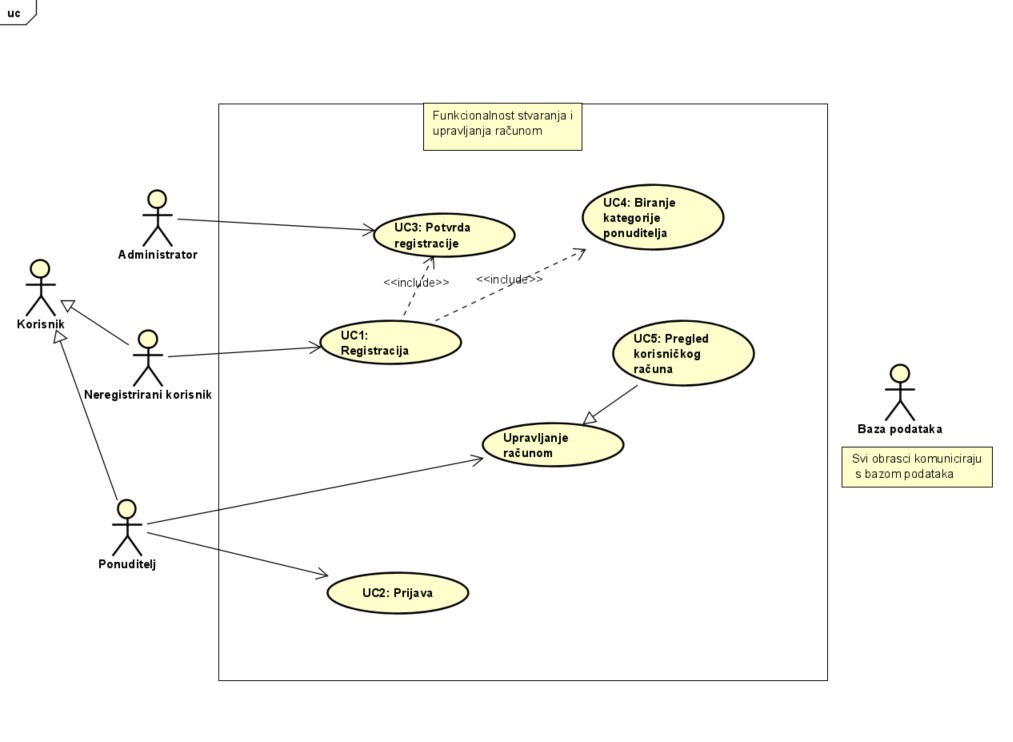
\includegraphics[width = \textwidth]{slike/DO1}
    					\caption{Dijagram obrazaca 1}
    					\label{fig:Dijagram obrazaca 1}
				\end{figure}

				\begin{figure}
    					\centering
    					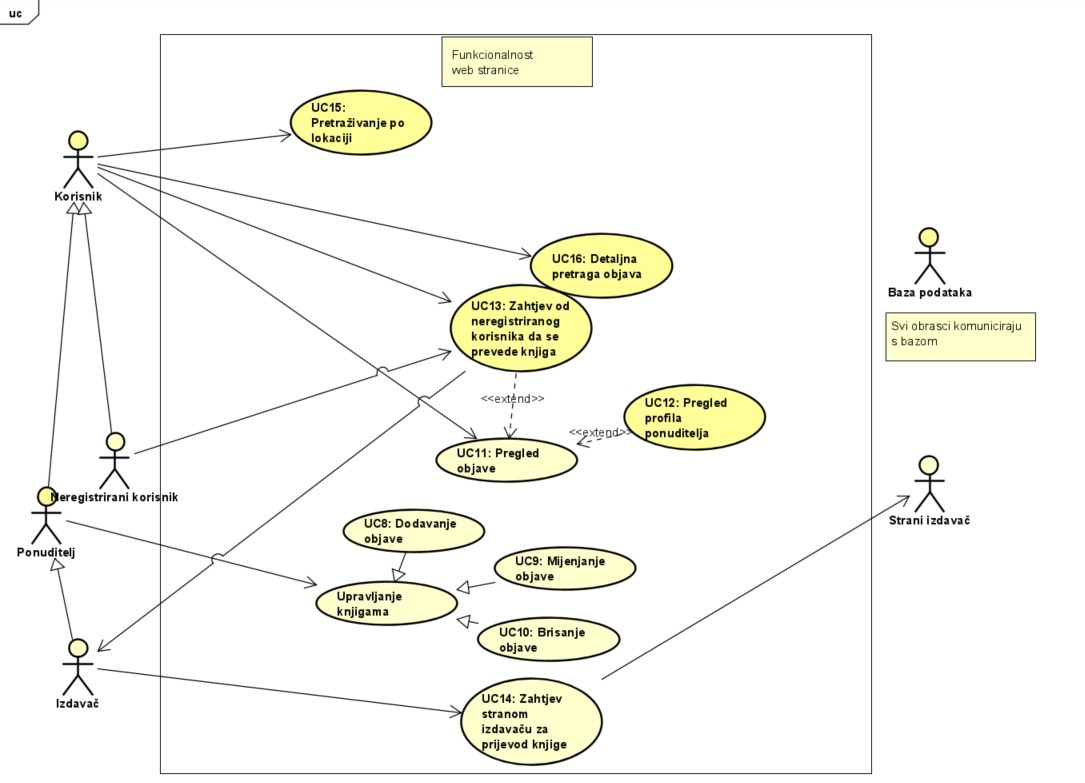
\includegraphics[width = \textwidth]{slike/DO2}
    					\caption{Dijagram obrazaca 2}
    					\label{fig:Dijagram obrazaca 2}
				\end{figure}
				\eject	
					
	
				
			\subsection{Sekvencijski dijagrami}
				
				\textbf{Obrazac uporabe UC15 – Pretraživanje po lokaciji i UC13 – Zahtjev da se prevede knjiga}\\\\
				Neregistrirani korisnik šalje zahtjev za pregled karte ponuditelja knjiga. Poslužitelj dohvaća ponuditelje knjiga iz baze i vraća prikaz karte sa označenim adresama ponuditelja. Korisnik odabire ponuditelja koji je izdavač. Poslužitelj dohvaća podatke o odabranom ponuditelju iz baze. Vraća korisniku listu svih knjiga dotičnog ponuditelja. Korisnik dodatno filtrira ponudu knjiga po želji. Korisnik traži prijevod od izdavača. U bazi podataka povećava se broj zatraženih prijevoda za tu knjigu.\\
				\begin{center}
				\begin{adjustbox}{max width=\textwidth}
					\begin{sequencediagram}
						\newthread{A}{Neregistrirani korisnik}{}
						\newinst[5]{B}{Poslužitelj}{}
						\newinst[5]{C}{Baza podataka}{}
						\begin{call}{A}{1: zatražiPrikazKarte()}{B}{Prikaz ponuditelja na karti}
							\begin{call}{B}{1.1: dohvatiPonuditelje()}{C}{Vrati ponuditelje}
							\end{call}
						\end{call}
						\postlevel
						\begin{call}{A}{2: odaberiPonuditelja()}{B}{Prikaz liste knjiga}
							\begin{call}{B}{2.1: dohvatiPodatkeOPonuditelju()}{C}{Vrati podatke o ponuditelju}
							\end{call}
						\end{call}
						\postlevel
						\begin{sdblock}{opt}{[Korisnik želi dodatno filtrirati knjige]}
							\begin{call}{A}{pretražiKnjige(značajke)}{B}{Prikaz liste knjiga}
								\begin{call}{B}{dohvatiFiltriraneKnjige(značajke)}{C}{Vrati listu knjiga}
								\end{call}
							\end{call}
						\end{sdblock}
						\postlevel
						\begin{call}{A}{3: odaberiKnjigu()}{B}{Prikaz podataka o knjizi}
							\begin{call}{B}{3.1: dohvatiPodatkeOKnjizi()}{C}{Vrati podatke o knjizi} 
							\end{call}
						\end{call}
						\postlevel
						\begin{messcall}{A}{3: zatražiPrijevod()}{B}
							\begin{messcall}{B}{3.1: spremiZahtjevZaPrijevodom()}{C}
							\end{messcall}
						\end{messcall}
						
					\end{sequencediagram}
				\end{adjustbox}
				\end{center}
				\eject
				
				\textbf{Obrazac uporabe UC1 – Registracija i UC3 – Potvrda registracije}\\\\
				Ponuditelj šalje zahtjev za registraciju. Poslužitelj sprema zahtjev u bazu. Administrator pregledava zahtjeve za registraciju i odobrava zahtjev našeg ponuditelja. Ponuditelj je uspješno registriran, pa ima pristup potpunoj funkcionalnosti svojeg korisničkog računa.\\
				\begin{center}
					\begin{adjustbox}{max width=\textwidth}
						\begin{sequencediagram}
							\newthread{A}{Ponuditelj}{}
							\newinst[5]{B}{Poslužitelj}{}
							\newinst[5]{C}{Baza podataka}{}
							\newthread{D}{Administrator}{}
							\begin{messcall}{A}{1: zatražiRegistraciju()}{B}
								\begin{messcall}{B}{1.1: spremiZahtjevZaRegistraciju()}{C}
								\end{messcall}
							\end{messcall}
							\begin{call}{D}{2: zatražiZahtjeveZaRegistraciju()}{B}{Prikaz zahtjeva za registraciju}
								\postlevel
								\begin{call}{B}{2.1: dohvatiZahtjeveZaRegistraciju()}{C}{Vrati zahtjeve za registraciju}
								\end{call}
								\postlevel
							\end{call}
							\postlevel
							\begin{messcall}{D}{3: odobriZahtjevZaRegistraciju()}{B}
								\postlevel
								\begin{messcall}{B}{3.1: spremiOdobrenogKorisnika()}{C}
								\end{messcall}
								\begin{messcall}{B}{3.2: izbrišiZahtjevZaRegistraciju()}{C}
								\end{messcall}
							\end{messcall}
						\end{sequencediagram}
					\end{adjustbox}
				\end{center}
				\eject
				
				\textbf{Obrazac uporabe UC8 – Dodavanje objave knjige}\\\\
				Preprodavač na stranici za dodavanje knjiga dodaje novi naslov. Poslužitelj sprema taj naslov u bazu pa ponuditelj dobiva opciju ponuditi primjerke tog naslova. Ponuditelj nudi primjerke tog naslova.\\
				\begin{center}
					\begin{adjustbox}{max width=\textwidth}
						\begin{sequencediagram}
							\newthread{A}{Preprodavač}{}
							\newinst[5]{B}{Poslužitelj}{}
							\newinst[5]{C}{Baza podataka}{}
							\begin{call}{A}{1: zatražiDodavanjeKnjiga()}{B}{Prikaz stranice za dodavanje knjiga}
								\begin{call}{B}{1.1: dohvatiPodatkeOPonuditelju()}{C}{Vrati podatke o ponuditelju}
								\end{call}
							\end{call}
							\postlevel
							\begin{messcall}{A}{2: dodajNaslov}{B}
								\begin{messcall}{B}{2.1: dodajNaslov()}{C}
								\end{messcall}
							\end{messcall}
							\begin{messcall}{A}{3: dodajPrimjerkeKnjige()}{B}
								\begin{messcall}{B}{3.1: dodajPrimjerkeKnjige()}{C}
								\end{messcall}
							\end{messcall}
						\end{sequencediagram}
					\end{adjustbox}
				\end{center}
				\eject
				
				\textbf{Obrazac uporabe UC16 - Detaljna pretraga objava knjiga i UC11 - pregled objave}\\\\
				Neregistrirani korisnik pretražuje knjige po sljedećim značajkama: naziv knjige, naziv autora, godina izdanja, redni broj izdanja, kategorija izdavača, žanr knjige, ISBN, oznaka vrste knjige. Poslužitelj postavlja upit prema bazi i vraća rezultat. Korisnik pregledava podatke pronađene knjige.\\
				\begin{center}
					\begin{adjustbox}{max width=\textwidth}
						\begin{sequencediagram}
							\newthread{A}{Neregistrirani korisnik}{}
							\newinst[5]{B}{Poslužitelj}{}
							\newinst[5]{C}{Baza podataka}{}
							\begin{call}{A}{1: pretražiKnjige(značajke)}{B}{Prikaz liste knjiga}
								
								\begin{call}{B}{1.1: dohvatiFiltriraneKnjige(značajke)}{C}{Lista knjiga}
								\end{call}
							\end{call}
							\postlevel
							\begin{call}{A}{2: odaberiKnjigu()}{B}{Prikaz podataka o knjizi}
								\begin{call}{B}{2.1: dohvatiPodatkeOKnjizi()}{C}{Podatci o knjizi}
								\end{call}
							\end{call}
						\end{sequencediagram}
					\end{adjustbox}
				\end{center}
				\eject
	
	
		\section{Ostali zahtjevi}
		
			
			 \begin{packed_item}
			 
			 \item Korisničko sučelje mora biti responzivno, dakle prilagođeno i stolnim računalima i mobilnim uređajima.
			 
			 \item Osnovne funkcionalnosti moraju biti jasno vidljive i dostupne u nekoliko klikova.
			 
			 \item Vrijeme odziva na obične naredbe treba biti manje od sekundu, a upiti bazi podataka moraju primiti odgovor za manje od pet sekundi.
			 
			 \item Web aplikacija mora biti implementirana objektno-orijentiranim jezikom.
			 
			 \item Sustav mora podržavati istovremen rad više korisnika.
			 
			 \item Cijene moraju biti u eurima, ali neka bude prikazana cijena i u kunama.
			 
			 \item Sustav mora informirati korisnika o nepravilnom korištenju.
			 
			 \item Mora biti omogućen pristup sustavu preko HTTPS-a.
			 
			 \item Veza s bazom podataka mora biti sigurna.
			 
			 	
			 \end{packed_item}
			 
			 
			
			 
			 
	\chapter{Arhitektura i dizajn sustava}
		
		\textbf{\textit{dio 1. revizije}}\\

		\textit{ Potrebno je opisati stil arhitekture te identificirati: podsustave, preslikavanje na radnu platformu, spremišta podataka, mrežne protokole, globalni upravljački tok i sklopovsko-programske zahtjeve. Po točkama razraditi i popratiti odgovarajućim skicama:}
	\begin{itemize}
		\item 	\textit{izbor arhitekture temeljem principa oblikovanja pokazanih na predavanjima (objasniti zašto ste baš odabrali takvu arhitekturu)}
		\item 	\textit{organizaciju sustava s najviše razine apstrakcije (npr. klijent-poslužitelj, baza podataka, datotečni sustav, grafičko sučelje)}
		\item 	\textit{organizaciju aplikacije (npr. slojevi frontend i backend, MVC arhitektura) }		
	\end{itemize}

	
		

		

				
		\section{Baza podataka}
			
			\textbf{\textit{dio 1. revizije}}\\
			
		\textit{Potrebno je opisati koju vrstu i implementaciju baze podataka ste odabrali, glavne komponente od kojih se sastoji i slično.}
		
			\subsection{Opis tablica}
			

				\textit{Svaku tablicu je potrebno opisati po zadanom predlošku. Lijevo se nalazi točno ime varijable u bazi podataka, u sredini se nalazi tip podataka, a desno se nalazi opis varijable. Svjetlozelenom bojom označite primarni ključ. Svjetlo plavom označite strani ključ}
				
				
				\begin{longtblr}[
					label=none,
					entry=none
					]{
						width = \textwidth,
						colspec={|X[6,l]|X[6, l]|X[20, l]|}, 
						rowhead = 1,
					} %definicija širine tablice, širine stupaca, poravnanje i broja redaka naslova tablice
					\hline \SetCell[c=3]{c}{\textbf{korisnik - ime tablice}}	 \\ \hline[3pt]
					\SetCell{LightGreen}IDKorisnik & INT	&  	Lorem ipsum dolor sit amet, consectetur adipiscing elit, sed do eiusmod  	\\ \hline
					korisnickoIme	& VARCHAR &   	\\ \hline 
					email & VARCHAR &   \\ \hline 
					ime & VARCHAR	&  		\\ \hline 
					\SetCell{LightBlue} primjer	& VARCHAR &   	\\ \hline 
				\end{longtblr}
				
				
			
			\subsection{Dijagram baze podataka}
				\textit{ U ovom potpoglavlju potrebno je umetnuti dijagram baze podataka. Primarni i strani ključevi moraju biti označeni, a tablice povezane. Bazu podataka je potrebno normalizirati. Podsjetite se kolegija "Baze podataka".}
			
			\eject
			
			
		\section{Dijagram razreda}
		
			\raggedright{Razred Knjiga predstavlja jednu knjigu koja se može pronaći na stranici. Razred Neregistrirani predstavlja korisnika koji može samo pretraživati knjige. Razred registrirani predstavlja korisnika koji sustav koristi za ponudu knjiga. Izdavač, Antikvarijat i Preprodavač su razredi koji predstavljaju različite vrste registriranog korisnika. Svaki registrirani korisnik je jedna od tih tri vrste i zbog toga je razred Registrirani apstraktan. Razred Ponuda predstavlja ponudu jedne knjige. Razred VrstaKnjige predstavlja vrstu svake knjige.}\\
			
			\begin{figure}[h]
				\centering
				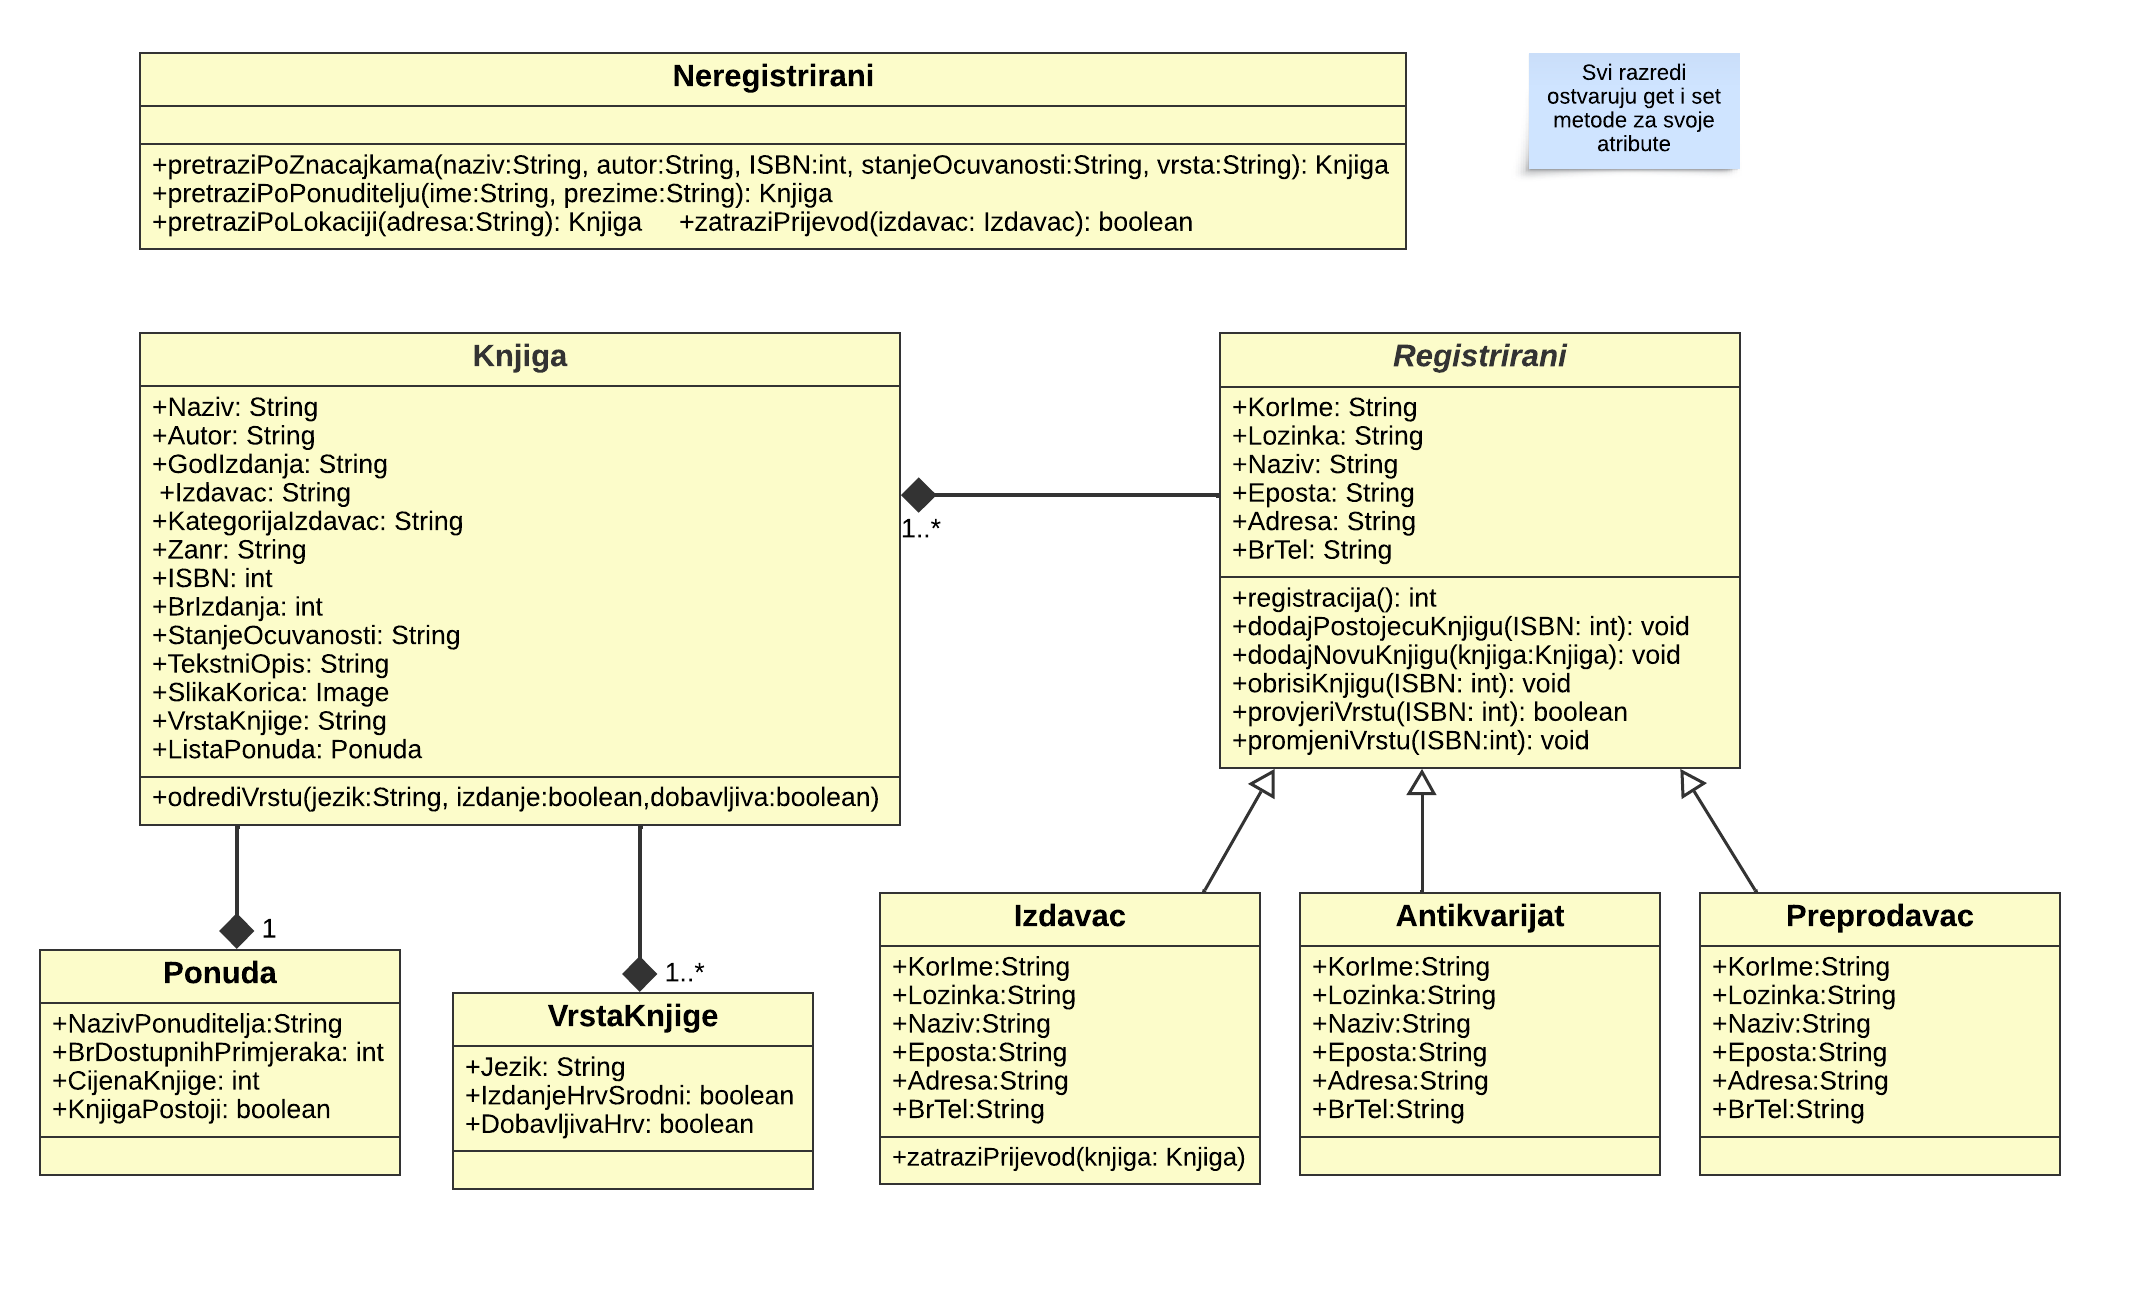
\includegraphics[width = \textwidth]{slike/dijagramKlasa.PNG}
				\caption{Dijagram razreda}
				\label{fig:enter-label}
			\end{figure}
			
			\textbf{\textit{dio 2. revizije}}\\			
			
			\textit{Prilikom druge predaje projekta dijagram razreda i opisi moraju odgovarati stvarnom stanju implementacije}
			
			
			
			\eject
		
		\section{Dijagram stanja}
			
			
			\textbf{\textit{dio 2. revizije}}\\
			
			\textit{Potrebno je priložiti dijagram stanja i opisati ga. Dovoljan je jedan dijagram stanja koji prikazuje \textbf{značajan dio funkcionalnosti} sustava. Na primjer, stanja korisničkog sučelja i tijek korištenja neke ključne funkcionalnosti jesu značajan dio sustava, a registracija i prijava nisu. }
			
			
			\eject 
		
		\section{Dijagram aktivnosti}
			
			\textbf{\textit{dio 2. revizije}}\\
			
			 \textit{Potrebno je priložiti dijagram aktivnosti s pripadajućim opisom. Dijagram aktivnosti treba prikazivati značajan dio sustava.}
			
			\eject
		\section{Dijagram komponenti}
		
			\textbf{\textit{dio 2. revizije}}\\
		
			 \textit{Potrebno je priložiti dijagram komponenti s pripadajućim opisom. Dijagram komponenti treba prikazivati strukturu cijele aplikacije.}
	\chapter{Implementacija i korisničko sučelje}
		
		
		\section{Korištene tehnologije i alati}
		
			
			 
			 Za timsku komunikaciju koristili smo WhatsApp\footnote{https://www.whatsapp.com/} koji nam je pružio brz i jednostavan medij. Za vizualizaciju i modeliranje sustava, Astah Professional\footnote{http://astah.net/editions/professional} bio je naš odabir, omogućio nam je izradu UML dijagrama koji su olakšali razumijevanje strukture i funkcionalnosti projekta.\\
			 
			 Git\footnote{https://git-scm.com/} je bio ključan u procesu upravljanja izvornim kodom, omogućavajući nam upravljanje inačicama i suradnju na projektu. Udruženi repozitorij projekta smješten na GitHub\footnote{https://github.com} platformi pružio je centralizirano mjesto za pohranu, pregled i praćenje promjena u kodu.\\
			 
			 Za razvoj softvera koristili smo Rider\footnote{https://www.jetbrains.com/rider/} integrirano razvojno okruženje (IDE) koje nam je omogućilo učinkovitiju izradu aplikacije.\\
			 
			 Na strani backenda, odabrali smo ASP.NET Core radni okvir\footnote{https://dotnet.microsoft.com/en-us/apps/aspnet/} u kombinaciji s jezikom C\#\footnote{https://docs.microsoft.com/en-us/dotnet/csharp/}, a za frontend smo se uz standardni HTML,\footnote{https://www.w3.org/html/} CSS\footnote{https://www.w3.org/Style/CSS/Overview.en.html} i JS\footnote{https://www.javascript.com/} oslonili na htmx\footnote{https://htmx.org/} radi njegove jednostavnosti.\\
			 
			 Baza podataka implementirana u PostgreSQL-u\footnote{https://www.postgresql.org/} smještena je na poslužitelju u oblaku Microsoft Azure\footnote{https://portal.azure.com/}.\newline
			
			
			\eject 
		
	
		\section{Ispitivanje programskog rješenja}
			
			\textbf{\textit{dio 2. revizije}}\\
			
			 \textit{U ovom poglavlju je potrebno opisati provedbu ispitivanja implementiranih funkcionalnosti na razini komponenti i na razini cijelog sustava s prikazom odabranih ispitnih slučajeva. Studenti trebaju ispitati temeljnu funkcionalnost i rubne uvjete.}
	
			
			\subsection{Ispitivanje komponenti}
			\textit{Potrebno je provesti ispitivanje jedinica (engl. unit testing) nad razredima koji implementiraju temeljne funkcionalnosti. Razraditi \textbf{minimalno 6 ispitnih slučajeva} u kojima će se ispitati redovni slučajevi, rubni uvjeti te izazivanje pogreške (engl. exception throwing). Poželjno je stvoriti i ispitni slučaj koji koristi funkcionalnosti koje nisu implementirane. Potrebno je priložiti izvorni kôd svih ispitnih slučajeva te prikaz rezultata izvođenja ispita u razvojnom okruženju (prolaz/pad ispita). }
			
			
			
			\subsection{Ispitivanje sustava}
			
			 \textit{Potrebno je provesti i opisati ispitivanje sustava koristeći radni okvir Selenium\footnote{\url{https://www.seleniumhq.org/}}. Razraditi \textbf{minimalno 4 ispitna slučaja} u kojima će se ispitati redovni slučajevi, rubni uvjeti te poziv funkcionalnosti koja nije implementirana/izaziva pogrešku kako bi se vidjelo na koji način sustav reagira kada nešto nije u potpunosti ostvareno. Ispitni slučaj se treba sastojati od ulaza (npr. korisničko ime i lozinka), očekivanog izlaza ili rezultata, koraka ispitivanja i dobivenog izlaza ili rezultata.\\ }
			 
			 \textit{Izradu ispitnih slučajeva pomoću radnog okvira Selenium moguće je provesti pomoću jednog od sljedeća dva alata:}
			 \begin{itemize}
			 	\item \textit{dodatak za preglednik \textbf{Selenium IDE} - snimanje korisnikovih akcija radi automatskog ponavljanja ispita	}
			 	\item \textit{\textbf{Selenium WebDriver} - podrška za pisanje ispita u jezicima Java, C\#, PHP koristeći posebno programsko sučelje.}
			 \end{itemize}
		 	\textit{Detalji o korištenju alata Selenium bit će prikazani na posebnom predavanju tijekom semestra.}
			
			\eject 
		
		
		\section{Dijagram razmještaja}
			
			\textbf{\textit{dio 2. revizije}}
			
			 \textit{Potrebno je umetnuti \textbf{specifikacijski} dijagram razmještaja i opisati ga. Moguće je umjesto specifikacijskog dijagrama razmještaja umetnuti dijagram razmještaja instanci, pod uvjetom da taj dijagram bolje opisuje neki važniji dio sustava.}
			
			\eject 
		
		\section{Upute za puštanje u pogon}
		
			\textbf{\textit{dio 2. revizije}}\\
		
			 \textit{U ovom poglavlju potrebno je dati upute za puštanje u pogon (engl. deployment) ostvarene aplikacije. Na primjer, za web aplikacije, opisati postupak kojim se od izvornog kôda dolazi do potpuno postavljene baze podataka i poslužitelja koji odgovara na upite korisnika. Za mobilnu aplikaciju, postupak kojim se aplikacija izgradi, te postavi na neku od trgovina. Za stolnu (engl. desktop) aplikaciju, postupak kojim se aplikacija instalira na računalo. Ukoliko mobilne i stolne aplikacije komuniciraju s poslužiteljem i/ili bazom podataka, opisati i postupak njihovog postavljanja. Pri izradi uputa preporučuje se \textbf{naglasiti korake instalacije uporabom natuknica} te koristiti što je više moguće \textbf{slike ekrana} (engl. screenshots) kako bi upute bile jasne i jednostavne za slijediti.}
			
			
			 \textit{Dovršenu aplikaciju potrebno je pokrenuti na javno dostupnom poslužitelju. Studentima se preporuča korištenje neke od sljedećih besplatnih usluga: \href{https://aws.amazon.com/}{Amazon AWS}, \href{https://azure.microsoft.com/en-us/}{Microsoft Azure} ili \href{https://www.heroku.com/}{Heroku}. Mobilne aplikacije trebaju biti objavljene na F-Droid, Google Play ili Amazon App trgovini.}
			
			
			\eject 
	\chapter{Zaključak i budući rad}
		
		Glavni izazov prilikom upravljanja projektom svakako je bila sklonost nedostatnoj komunikaciji koju se najučinkovitije suzbilo češćim pozivima umjesto slanja poruka.
		
		Osim toga bilo je zahtjevno raspodijeliti zadatke tako da se ne preopterete članovi koji rade na programskoj implementaciji, ali istovremeno da ne bi netko primjerice morao proučavati backend da napravi dijagram razreda kada bi ga lakše backendaš napravio.
		
		Jedan od izazova bilo je i popravljanje korisničkog sučelja koje bi redovito bilo strgano promjenama na backendu. Nismo smislili rješenje za tu situaciju osim popravljanja dok ne proradi.
		
		Nadvladavanjem tih i drugih izazova stekli smo razna iskustva, svatko pojedinačno u tehnologiji kojom je baratao, ali i ono glavno, iskustvo timskog rada i poteškoća organizacije i učinkovite suradnje.
		
		Sve u svemu, iskustvo rada u timu na stvarnom projektu približilo nam je stvarnost programerskog rada.
		
		\eject 
	\chapter*{Popis literature}
		\addcontentsline{toc}{chapter}{Popis literature}
	 	
		
		\begin{enumerate}
			
			
			\item  Programsko inženjerstvo, FER ZEMRIS, \url{http://www.fer.hr/predmet/proinz}
			
			\item  Overleaf,
			\url{https://www.overleaf.com/}
			
			\item  \LaTeX\ WikiBook,
			\url{https://en.wikibooks.org/wiki/LaTeX/}
			
			\item  \LaTeX\ Stack Exchange,
			\url{https://tex.stackexchange.com/}
			
			\item  Lucidchart,
			\url{https://www.lucidchart.com/pages/}
			
		\end{enumerate}
		
		 
	
	
	\begingroup
	\renewcommand*\listfigurename{Indeks slika i dijagrama}
	%\renewcommand*\listtablename{Indeks tablica}
	%\let\clearpage\relax
	\listoffigures
	%\vspace{10mm}
	%\listoftables
	\endgroup
	\addcontentsline{toc}{chapter}{Indeks slika i dijagrama}


	
	\eject 
		
	\chapter*{Dodatak: Prikaz aktivnosti grupe}
		\addcontentsline{toc}{chapter}{Dodatak: Prikaz aktivnosti grupe}
		
		\section*{Dnevnik sastajanja}
		
		\textbf{\textit{Kontinuirano osvježavanje}}\\
		
		 \textit{U ovom dijelu potrebno je redovito osvježavati dnevnik sastajanja prema predlošku.}
		
		\begin{packed_enum}
			\item  sastanak
			
			\item[] \begin{packed_item}
				\item Datum: u ovom formatu: \today
				\item Prisustvovali: I.Prezime, I.Prezime
				\item Teme sastanka:
				\begin{packed_item}
					\item  opis prve teme
					\item  opis druge teme
				\end{packed_item}
			\end{packed_item}
			
			\item  sastanak
			\item[] \begin{packed_item}
				\item Datum: u ovom formatu: \today
				\item Prisustvovali: I.Prezime, I.Prezime
				\item Teme sastanka:
				\begin{packed_item}
					\item  opis prve teme
					\item  opis druge teme
				\end{packed_item}
			\end{packed_item}
			
			%
			
		\end{packed_enum}
		
		\eject
		\section*{Tablica aktivnosti}
		
			\textbf{\textit{Kontinuirano osvježavanje}}\\
			
			 \textit{Napomena: Doprinose u aktivnostima treba navesti u satima po članovima grupe po aktivnosti.}

			\begin{longtblr}[
					label=none,
				]{
					vlines,hlines,
					width = \textwidth,
					colspec={X[7, l]X[1, c]X[1, c]X[1, c]X[1, c]X[1, c]X[1, c]X[1, c]}, 
					vline{1} = {1}{text=\clap{}},
					hline{1} = {1}{text=\clap{}},
					rowhead = 1,
				} 
			
				\SetCell[c=1]{c}{} & \SetCell[c=1]{c}{\rotatebox{90}{\textbf{Dominik Agejev }}} & \SetCell[c=1]{c}{\rotatebox{90}{\textbf{Marko Haralović }}} &	\SetCell[c=1]{c}{\rotatebox{90}{\textbf{Ivan Skukan }}} & \SetCell[c=1]{c}{\rotatebox{90}{\textbf{Lovro Galiot }}} &	\SetCell[c=1]{c}{\rotatebox{90}{\textbf{Marin Lovrinović }}} & \SetCell[c=1]{c}{\rotatebox{90}{\textbf{Niko Vidović }}} &	\SetCell[c=1]{c}{\rotatebox{90}{\textbf{Tvrtko Tomić }}} \\  
				Upravljanje projektom 		&  &  &  &  &  &  & \\ 
				Opis projektnog zadatka 	&  &  &  &  &  &  & \\ 
				
				Funkcionalni zahtjevi       &  &  & 7 & 3 &  &  &  \\ 
				Opis pojedinih obrazaca 	&  &  & 3 & 2 &  &  &  \\ 
				Dijagram obrazaca 			&  &  & 4 & 1 &  &  &  \\ 
				Sekvencijski dijagrami 		&  &  &  &  &  &  &  \\ 
				Opis ostalih zahtjeva 		&  &  &  &  &  &  &  \\ 

				Arhitektura i dizajn sustava	 &  &  &  &  &  &  &  \\ 
				Baza podataka				&  &  &  &  &  &  &   \\ 
				Dijagram razreda 			&  &  &  &  &  &  &   \\ 
				Dijagram stanja				&  &  &  &  &  &  &  \\ 
				Dijagram aktivnosti 		&  &  &  &  &  &  &  \\ 
				Dijagram komponenti			&  &  &  &  &  &  &  \\ 
				Korištene tehnologije i alati 		&  &  &  &  &  &  &  \\ 
				Ispitivanje programskog rješenja 	&  &  &  &  &  &  &  \\ 
				Dijagram razmještaja			&  &  &  &  &  &  &  \\ 
				Upute za puštanje u pogon 		&  &  &  &  &  &  &  \\  
				Dnevnik sastajanja 			&  &  &  &  &  &  &  \\ 
				Zaključak i budući rad 		&  &  &  &  &  &  &  \\  
				Popis literature 			&  &  &  &  &  &  &  \\  
				&  &  &  &  &  &  &  \\ \hline 
				\textit{Dodatne stavke kako ste podijelili izradu aplikacije} 			&  &  &  &  &  &  &  \\ 
				Izrada početne stranice			        &  &  & 2 & 3 &  &  &  \\  
                Izrada stranica za objave               &  &  & 1 & 3 &  &  &  \\
                Izrada stranice za novu objavu          &  &  & 1 & 2 &  &  &  \\  
                Izrada stranice za login i registraciju &  &  & 4 & 1 &  &  &  \\ 
                Izrada stranice za pregled računa       &  &  & 2 & 2 &  &  &  \\  
                Izrada skripti za funkcionalnost stranice &  &  & 4 & 6 &  &  &  \\  
                Omogućavanje responzivnosti stranice    &  &  & 1 & 3 &  &  &  \\ 
                
				\textit{izrada baze podataka} 		 	&  &  &  &  &  &  & \\  
				\textit{spajanje s bazom podataka} 		&  &  &  &  &  &  &  \\ 
				\textit{back end} 							&  &  &  &  &  &  &  \\  
				 							&  &  &  &  &  &  &\\ 
			\end{longtblr}
					
					
		\eject
		\section*{Dijagrami pregleda promjena}
		
		\textbf{\textit{dio 2. revizije}}\\
		
		\textit{Prenijeti dijagram pregleda promjena nad datotekama projekta. Potrebno je na kraju projekta generirane grafove s gitlaba prenijeti u ovo poglavlje dokumentacije. Dijagrami za vlastiti projekt se mogu preuzeti s gitlab.com stranice, u izborniku Repository, pritiskom na stavku Contributors.}
		
	


\end{document} %naredbe i tekst nakon ove naredbe ne ulaze u izgrađen dokument 


